\documentclass[10pt,a4paper]{article}
\usepackage{times}                       % 使用 Times New Roman 字体
\usepackage{xeCJK}%CJK,CJKnumb,CJKulem}         % 中文支持宏包
\usepackage{color}                       % 支持彩色

\usepackage{comment}
\usepackage{amsmath}
\usepackage{amssymb}
\usepackage{amsthm}
\usepackage{amscd}
\usepackage{graphicx}
\usepackage{indentfirst}
\usepackage{titlesec}
\usepackage[top=25.4mm, bottom=25.4mm, left=31.7mm, right=32.2mm]{geometry}

%页面设置
%\begin{document}%CJK*}{GBK}{hei}
%\theoremstyle{definition}
%\newtheoremstyle{mythm}{1.5ex plus 1ex minus .2ex}{1.5ex plus 1ex minus .2ex}
%   {\kai}{\parindent}{\song\bfseries}{}{1em}{}
\newtheoremstyle{mythm}{1ex}{1ex}%定理环境的上下间距.
{\CJKfamily{song}}{\parindent}{\CJKfamily{hei} \bf}{}{1em}{}%定理内容为宋体, 缩进, 定理名称为黑粗体
\theoremstyle{mythm}%设置定理环境
\newtheorem{thm}{定理~}[section]
\newtheorem{lem}[thm]{引理~}
\newtheorem{pro}[thm]{性质~}
\newtheorem{fact}[thm]{Fact}
\newtheorem{prop}[thm]{命题~}
\newtheorem{ques}[thm]{问题~}
\newtheorem{cor}[thm]{推论~}
\newtheorem{de}[thm]{定义~}
\newtheorem{rem}[thm]{注记~}
\numberwithin{equation}{section}
%\end{document}%CJK*}
\renewcommand\refname{\CJKfamily{hei}参考文献}
%\renewcommand{\abstractname}{摘要}
%%%%%%%%%%%%%%%%下面几行用于改变证明环境的定义
\makeatletter
\renewenvironment{proof}[1][\proofname]{\par
\pushQED{\qed}%
\normalfont \topsep6\p@\@plus6\p@ \labelsep1em\relax
\trivlist
\item[\hskip\labelsep\indent
\bfseries #1]\ignorespaces
}{%
\popQED\endtrivlist\@endpefalse
}
\makeatother
%%%%%%%%%%%%%%(http://latex.yo2.cn)
\renewcommand{\proofname}{\CJKfamily{hei}证明}

\renewcommand{\thefootnote}{\fnsymbol{footnote}}
%\titleformat{\section}{\CJKfamily{hei} }{\arabic{section}{1em}{}
\titleformat{\section}{\large \bf \CJKfamily{hei} }{{\bf \thesection\space}}{0pt}{}

\begin{document}
%\setlength{\baselineskip}{1ex}%设置行距
\setlength{\abovedisplayskip}{1ex} %设置公式上边间距
\setlength{\belowdisplayskip}{1ex} %设置公式下边间距
%\begin{xeCJK}%{GBK}{song}

\author{马国芳11621003}                                 % 作者
\title{上下文感知的协同主题回归社会矩阵分解的推荐系统}              % 题目
\maketitle                                           % 生成标题

\section{引言}
%\clearpage % 换页,\newpage也可以,推荐\clearpage
文本介绍《Context-Aware Collaborative Topic Regression with Social Matrix Factorization for Recommender Systems》$^{[1]}$(AAAI)。在这个社交大数据时代,主流的在线社交网站,如Epinions,推特,和Last.fm等,已成为用户之间分享信息的主要平台。这些社交网络不仅包含大量的基本信息,还包含了上下文、社会关系、物品内容等有价值的信息。这三种类型的信息已经被证明是有价值的,和用户对物品的评分结合,可以建立更准确的推荐系统(RSS)。然而,据我们所知,现有的研究没有将完全结合这些不同类型的信息,以进一步提高推荐质量。
\paragraph{问题}协同过滤仅使用用户-物品评分信息,存在数据稀疏性和评分不平衡的问题,为了解决上述问题,加入我们可以以下信息:上下文、社会关系、物品内容、物品内容与社会关系。
 \paragraph{挑战}第一个挑战是如何系统的组合各类信息来优化预测结果。第二个挑战是如何充分利用每种信息,使他们可以最大的作用。
 \paragraph{贡献}本文结合评分、上下文(用户上下文、物品上下文、评分上下文)、社会关系、物品内容来建立了一个更准确的推荐系统。本文使用谱聚类而不是决策树来进行矩阵分组,使我们的方法可以同时处理分类的上下文和连续上下文。本文提出了新的分层贝叶斯模型,考虑社会关系,基于用户和信任他们的人类给用户分配不同的先验,来充分利用社交信任关系。

\section{相关知识}
\subsection{矩阵分解(MF)}
就在附近是最普遍的方法之一,它将用户项目评分矩阵分解为一个用户特征矩阵和一个物品特征矩阵。然后用二次正则化项来最目标函数的平方和。社会矩阵分解将社会关系融入MF以提高推荐算法的性能。最常用的方法是在方程中添加社交正则项来约束一个用户和另一个用户之间的爱好差异。例如,Jamali and Ester 使用用户的直接邻居的平均潜在特征作为用户的唯一先验,基于假设:一个用户的爱好接近用户的朋友的平均爱好。我们把这个术语简称MFTP。然而,MFTP不区别对待用户之间的信任值和信任他们的人。在本文的工作中,我们分配不同的先验给用户基于用户之间的信任值和那些他们信任的人来充分利用社会的信任关系。
\subsection{上下文感知的推荐方法}
上下文信息,如年龄、时间、和位置,已被证明可以用来建立更精确的RSS。最近的研究主要集中在利用上下文进行用户项目分组。分组已被证明是进一步提高许多流行的CF方法推荐性能的一种有效方式。然而,许多研究用决策树给具有相似上下文的用户-物品分组,因此他们只能处理分类情况。在我们的工作中,我们提出了使用谱聚类的用户项目分组,它可以同时处理分类和连续的上下文。
\subsection{基于主题模型的推荐方法}
基于原始文本的分层贝叶斯,主题模型被用来发现文档中的主题集合。作为最简单的主题模型,LDA已被用于许多应用,包括RSS。最近的研究集中在使用LDA来挖掘有用和丰富的文本内容。Wang and Blei提出了合作主题回归CTR,结合MF的概率主题模型的优点。CTR与SoRec联合来获得一个一致且紧凑的特征表达,叫CTE-SMF。因为CTR-SMF使用SOREC来开发社会关系,它不区别对待所有的朋友。此外,CTR-SMF忽略了另一重要信息来源:上下文。在本文中,我们将集中在未来的这两个缺点。

\section{方法概述}
%\CJKfamily{fs}
%中文部分,可以中英文混合
%
%\CJKfamily{hei}
%中文部分,可以中英文混合
%
%\CJKfamily{li}
%中文部分,可以中英文混合
%
%\CJKfamily{kai}
%中文部分,可以中英文混合
%
%\CJKfamily{song}
%中文部分,可以中英文混合
\subsection{准备工作}
我们将传统的二维空间User× Item变为三维空间User× Item×Context。在线社交网络的上下文信息分类包括
(1)用户上下文,它描述了用户的特性,(2)项目上下文,它描述了一个项目的特点,(3)评分上下文,这代表了用户对物品评分时提供的附加信息。例如,在Epinions,用户上下文包括:(1)访问次数,(2)评论数(3)被信任人的数量,(4)信任人的数量(5)用户的平均评分。物品上下文包括:(6)物品类别,(7)物品的平均评分,以及(8)评论者的数量。评级的背景包括:(9)一天中的某时间,(10)一周中的某天,和(11)评论质量级。
\subsection{动机}
我们的方法可以同时处理评分、上下文、社交关系、物品内容。
首先采用光谱聚类对具有相似上下文的用户和物品分组。
然后在每个用户物品分组中,我们应用我们所提出的分层贝叶斯模型进行预测。 
我们的模型是一个组合的LDA和SMF。使用LDA挖掘物品的内容信息,使用SMF处理评分和社会信任关系。 
然而,不像CTR-SMF对整个社会的信任网络只放单个先验,我们的模型基于用户与信任他的人之间的信任值给每个用户单独设置一个先验来处理社交关系,因此,我们的方法可以对所有的用户是不同的,比现有的模型更符合实际情况。
\subsection{基于上下文的用户-物品分组}
并不是所有的上下文都会影响推荐。首先,我们采用统计测试,调查的上下文和评分之间的相互作用,来选择有用的上下文,我们选择了以下上下文对用户物品分组:(2)评论数量,(5)用户平均评分、(6)物品的类别,和(7)物品的平均评级。
接下来,我们使用谱聚类做用户物品分组。第一步是将所有选定的上下文规范化为同一范围,如[ 0,5 ]。二步是计算基于上下文的相似度矩阵。最后一步是使用相似度矩阵,并设置一个聚类数$ \iota   $,以运行谱聚类。聚类后,我们得到的$ \iota   $个用户物品评分子矩阵,我们可以利用我们所提出的分层贝叶斯模型预测。

\subsection{本文方法}
我们提出的模型C-CTR-SMF2是分层贝叶斯模型,共同学习用户和物品的潜在空间。C-CTR-SMF2是结合LDA和SMF。我们使用LDA挖掘物品的内容信息,使用SMF处理评分和社会信任网络。


内容参数$ \lambda_v$平衡物品的内容信息对模型性能的贡献,$\lambda_v = \infty $时C-CTR-SMF2倾向LDA。
社会参数$ \lambda_f$F平衡社会关系对模型性能的贡献,$\lambda_f = 0 $时C-CTR-SMF2倾向CTR。
因此,LDA和CTR是我们模型的特殊情况。
不像CTR-SMF对整个社会的信任网络只放单个先验,我们的模型基于用户与信任他的人之间的信任值给每个用户单独设置一个先验来处理社交关系。
由于在方程(3)的社会正规化术语显示,这些功能让我们的模型充分利用社会信任网络
$$ \lambda_f{\sum}_{i=1}^I{\sum}_{f\in{N_i}}T_{if}{||U_i-U_f||}^2  \eqno{(3)}$$

模型生成过程如下

1、对所有的用户$u_1,...,u_i,...,u_I$,提取用户潜在向量集,$U \sim p(U)$
\[p(U)\propto N(0,\lambda_u^{-1}) {\prod}^I_{i=1} {\prod}_{f\in N_i} N(U_f,\lambda_f^{-1} T_{if}^{-1})\]\

2、对每个物品$j$

(a)提取主题比例$\theta_j \sim Dirichlet(\alpha)$

(b)提取物品潜在偏移$\epsilon_j \sim N(0,\lambda_v^{-1})$,则物品潜在向量为$V_j = \epsilon_j + \theta_j$

(c)对每个单词$w_{jn}$

i.提取主题匹配$z_{jn} \sim Mult(\theta)$

ii.提取单词$w_{jn}\sim Mult(\beta_{z_{jn}})$

3、对每个用户-物品对$(i,j)$,提取评分
\[R_{ij}\sim N(U_i^T V_j,c_{ij}^{-1})\]\

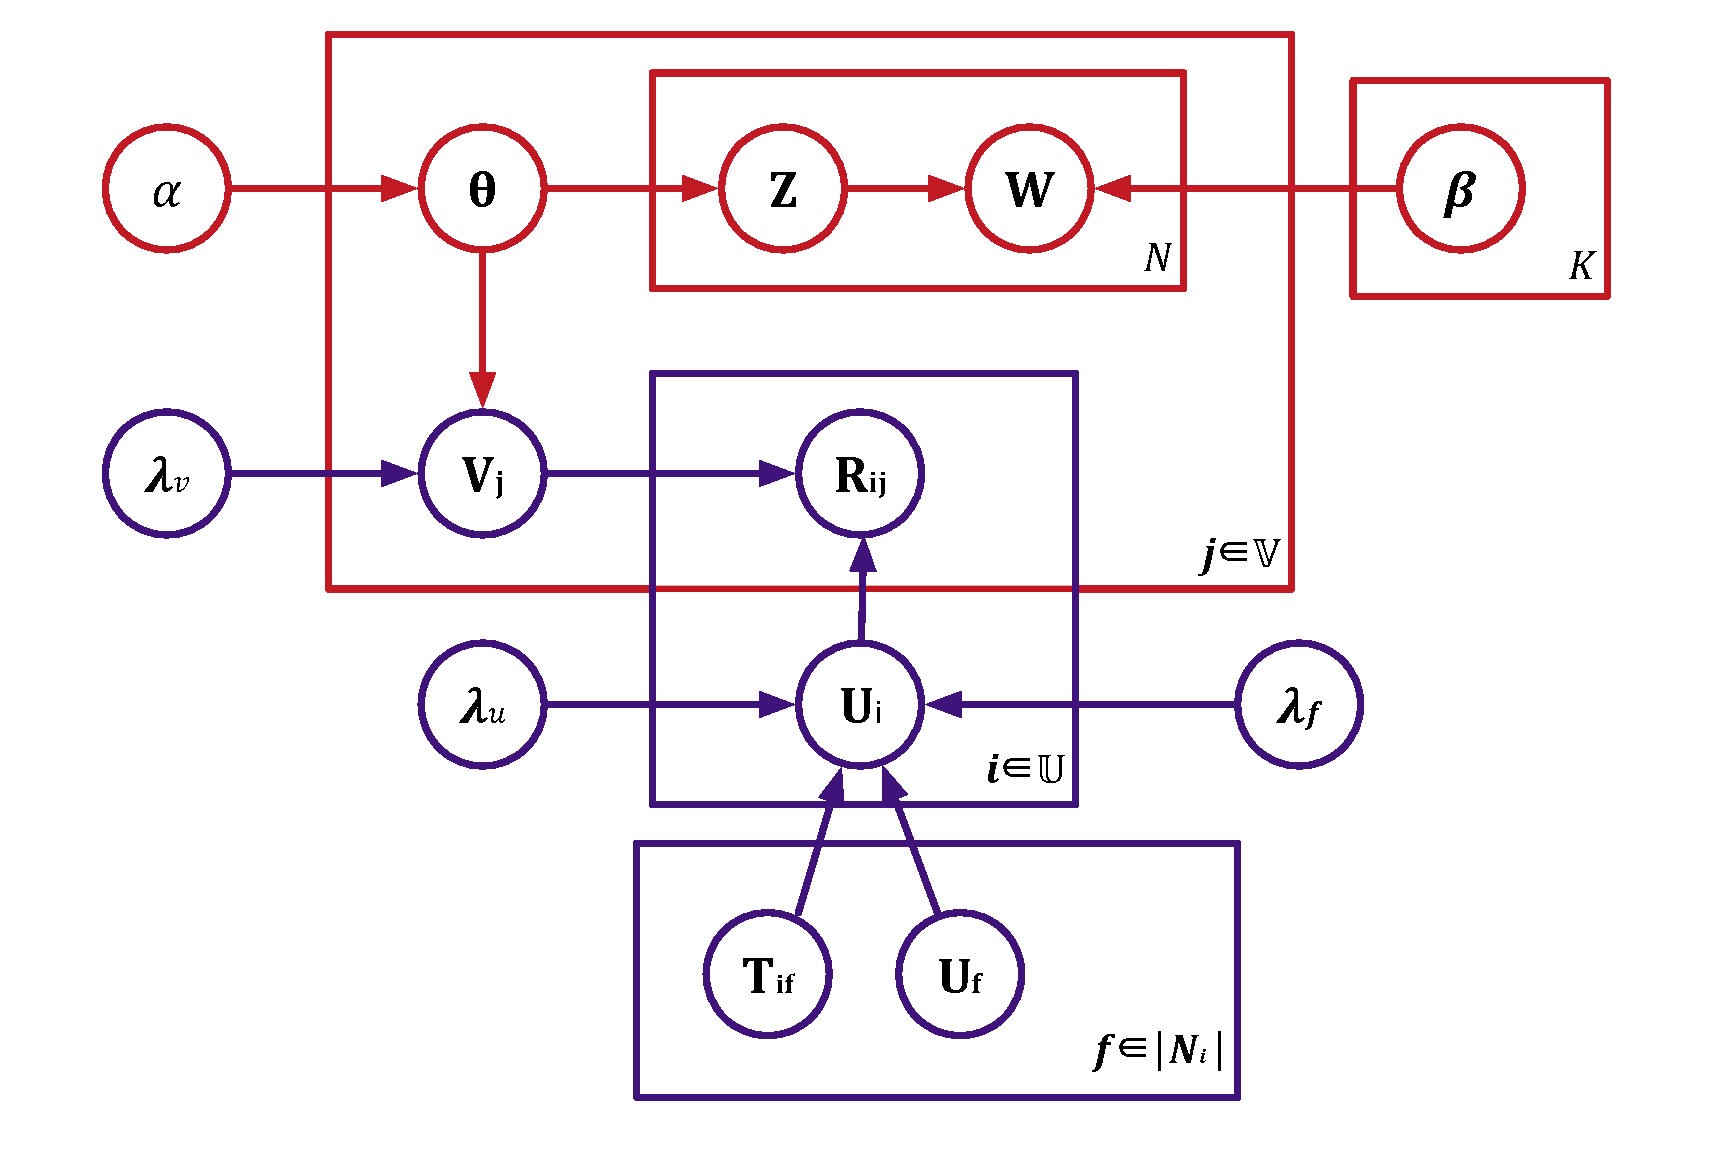
\includegraphics[width=5in]{figure1.eps} 

图1:我们提出的模型c-ctr图形模型素。LDA部分显示为红色,和SMF的部分显示在紫。

观察到的评分的条件分布可以表示为
\[p(R|U,V,\sigma_R^2) = {\prod}_{i=1}^I {\prod}_{j=1}^J{[N(R_{ij}|U_i^T V_j),\sigma_R^2)]}^{I_{ij}^R}\]\

其中$I_{ij}^R$是一个指示函数,当用户$i$对物品$j$有评分,它为1,否则为0

用户潜在向量$U_i$有两个部分的因素:期望值为零值高斯先验,避免过拟合,和给定用户直接邻居潜在特征的用户潜在特征的条件分布。因此,
\[p(U|U_f,T,\sigma_U^2,\sigma_T^2) \propto p(U|\sigma_U^2) \times {\prod}_{i=1}^I {\prod}_{f\in N_i} p(U|U_f,T_{if}^{-1}\sigma_T^2)\]\


物品特征向量$V_j$由CTR的一个键属性生成,它可以表现为
\[p(V|\sigma_V^2) \sim N(\theta_j,\lambda_v^{-1}I_k)\]

使用贝叶斯推理,我们可以通过给定的用户物品评分矩阵和社会信任矩阵来推断出以下公式的潜在特征向量的后验概率:
\[p(U,V|R,T,\sigma_R^2,\sigma_U^2,\sigma_V^2,\sigma_T^2) \propto p(R|U,V,\sigma_R^2) \times p(U|U_f,T,\sigma_U^2,\sigma_T^2) \times p(V|\sigma_V^2)\]
\subsection{学习参数}
直接计算$U_i,V_i,\theta_j$的后验是棘手的,我们开发了一个变化的EM算法来学习的最大后验估计。最大化后验在两个具有固定超参数的潜在特征相当于最大化以下U,V,$\theta_{1:J},\lambda_u,\lambda_v,\lambda_f,\beta$ 的完全对数似然

 \begin{equation}
\begin{split}
L = -\frac{\lambda_u}{2}{\sum}_i U_i^TU_i - \frac{\lambda_u}{2}{\sum}_j(V_j-\theta_j)^T(V_j - \theta_j) \\
+{\sum}_j {\sum}_n log({\sum}_k \theta_{jk}\beta_{k,w_{jn}}) \\
-{\sum}_{ij}\frac{c_{ij}}{2}(R_{ij}-U_i^T V_j)^2\\
-\frac{\lambda_f}{2}{\sum}_i{\sum}_{f\in N_i} T_{if}(U_i-U_f)^T(U_i-U_f
\end{split}
\end{equation}

其中$\lambda_u = \sigma_R^2/\sigma_U^2,\lambda_v = \sigma_R^2/\sigma_V^2,\lambda_f = \sigma_R^2/\sigma_T^2$和狄利克雷先验$(\alpha)$被设置为1。
$c_{ij}$是评分$R_{ij}$的置信参数。我们使用坐标下降来优化这个函数,即,通过迭代优化MF变量${U_i,V_j}$和主题的比例$\theta_j$。$U_i$和$V_j$的最大化以MF同样的方式。已知$\theta_j$的当前估计,将$L$关于$U_i$和$V_j$的梯度设置为0
$$U_i\gets(VC_iV^T + \lambda_uI_K +\lambda_fT_i1_II_K)^{-1}(\lambda_fUT_i^T + VC_iR_i)\eqno{(4)}$$
$$V_j\gets(UC_jU^T + \lambda_vI_K)^{-1}(UC_jR_j + \lambda_v\theta_j)\eqno{(5)}$$

公式(4)表示社交信任比例$T_i$影响用户潜在向量$U_i$,$\lambda_f$如何如何平衡这个影响。
当入$\lambda_f = 0$,我们的模型趋向去CTR(用物品内容和评分来进行预测),当$\lambda_f = \infty $,我们的模型只使用社交关系来对用户喜好进行建模。在其他情况下,我们的模型融合物品内容、评分和社会关系来进行预测。
公式(5)表示了主题比例如何影响物品隐藏向量$V_j$,$\lambda_v$如何平衡这个影响。当$\lambda_v = 0$,我们的模型只使用评分来进行预测。当$\lambda_v = \infty $,我们的模型只使用物品内容来进行预测,因此我们的模型趋向LDA。

给定$U$和$V$,我们现在学习了主题比例$\theta_j$,我们先定义$q(z_{jn}=k)=\Phi_{jnk}$,然后我们分开包含$\theta_j$的项,并运用詹森不等式,


 \begin{equation}
\begin{split}
L(\theta_j) \ge -\frac{\lambda_v}{2}(V_j-\theta_j)^T(V_j-\theta_j)+{\sum}_n{\sum}_k\Phi_{jnk}\\
(log\theta_{jk}\beta_{k,w_{jn}} - log\Phi_{jnk}) = L(\theta_j,\Phi_j)
\end{split}
\end{equation}

其中$\Phi_j = {\Phi_{jnk}}_{n=1,k=1}^{N\times K},N,j,\Phi_{jnk}$,$N$是物品$j$的内容字数,最佳的$\Phi_{jnk}$满足$\Phi_{jnk}\propto\theta_{jk}\beta_{k,w_{jn}}$。因此$L(\theta_j,\Phi_j)$给定了$L(\theta_j)$的最低下限。
然后投影梯度(Bertsekas,,1999)可应用于$\theta_j,$,坐标下降可用于优化其他参数的优化,如$U,V,\theta_{1:J},\Phi_{1:J}$。最后,通过估计$U,V,\Phi$,我们可以最优化$\beta$,
$$\beta_{kw}\propto{\sum}_j{\sum}_n\Phi_{jnk}1[w_{jn}=w]$$

通过最优化参数$U^*,V^*,{\theta_{1:J}}^*,\beta^*$,我们的模型可以用来进行预测和推荐。

$${R_{ij}}^* \approx {U_i^*}^TV_j^*$$


\section{实验结果}
在这一节中,我们将介绍对我们的方法性能进行评估的综合性实验。我们使用一个Epinions数据集进行的实验,帮助我们回答两个关键问题:(1)六个国家的最先进的RSS相比,我们的模型表现的如何?(2)在何种程度上做评级、背景、社会关系和项目内容,有助于获得更好的表现?
\subsection{数据集}
Epinions.com是分享产品相关知识的消费者意见网站。Epinions成员在可以评论物品(例如,食品,书籍,和电子产品)和并给物品打分1-5。同时,Epinions成员可以限制自己的信任网络,一组“评论者的评论,他们的评论被认为是有价值的。“Epinions还提供用户、物品和评分上下文。因此,对社会推荐实验Epinions是理想的数据源。

在我们的实验中使用的数据集由3474个用户,每个人都至少评论了6850个物品中的一个,共有77267个评论和37587个信任声明。用户物品矩阵的密度约为0.08\%。对于每一个物品,我们使用所有的优点,缺点和底线作为其内容,形成了59084个不同的术语。
\subsection{对比算法}

我们把我们所提出的方法C-CTR-SMF2与六个的推荐方法进行比较,每一个都是在其领域有前途的的方法。

PMF是基本的MF方法,只考虑评分。
SoReg (Ma et al., 2011)基于社交信任,同时考虑评分和社交关系的方法
fLDA (Agarwal and Chen, 2010)是个性化的sLDA,同时考虑上下文和物品内容
CTR (Wang and Blei, 2011)是一个基于主题模型的推荐模型,包含评分和物品内容。
CTR-SMF (Purushotham, Liu, and Kuo, 2012) 是一个组合的CTR和SOREC,包含评分、物品内容和社会关系,并采用入q来平衡CTR和SOREC效果。
SoCo (Liu and Aberer, 2013) 是一个模型,利用随机决策树来进行基于上下文的用户物品分组,并结评分,社会关系,和分类上下文。

\subsection{度量方法}
在我们的实验中,我们将数据集分成两个部分:训练数据集(80\%)和测试数据集(20\%)。我们用三个指标来衡量各种推荐模型的性能:召回率,平均绝对误差(MAE)、均方根误差(RMSE)。所有这三个是常用的指标,用于评估性能的预测。
\subsection{参数的选择与分析}
我们用五倍交叉验证发现,$K = 6,\lambda_u = \lambda_v = 0.1,a = 1,b = 0.01$提供最佳性能在MF方法。注意,$a$和$b$($a>b>0$)是置信参数$c_{i,j}$的调节参数。对SoCo,我们把决策树的数量和树的高度设置为3。我们还用五倍交叉验证发现CTR提供最佳性能时,$K = 20,\lambda_u = 0.1,a = 1,b = 0.01$,和CTR-SMF提供最佳性能时,$K = 15,\lambda_u = 0.1,a = 1,b = 0.01$。在这一部分后,我们将调节内容参数$\lambda_v$来学习它对CTR性能的影响。我们也会改变内容参数$\lambda_v$和社会参数$\lambda_q$,研究其对CTR-SMF性能的影响。我们的方法C-CTR-SMF2,就像CTR,我们设置$K = 20,\lambda_u = 0.1,a = 1,b = 0.01$,调节不同的谱聚类数$\iota$,内容参数$\iota$和社会参数$\lambda_f$,研究其对模型性能的影响。

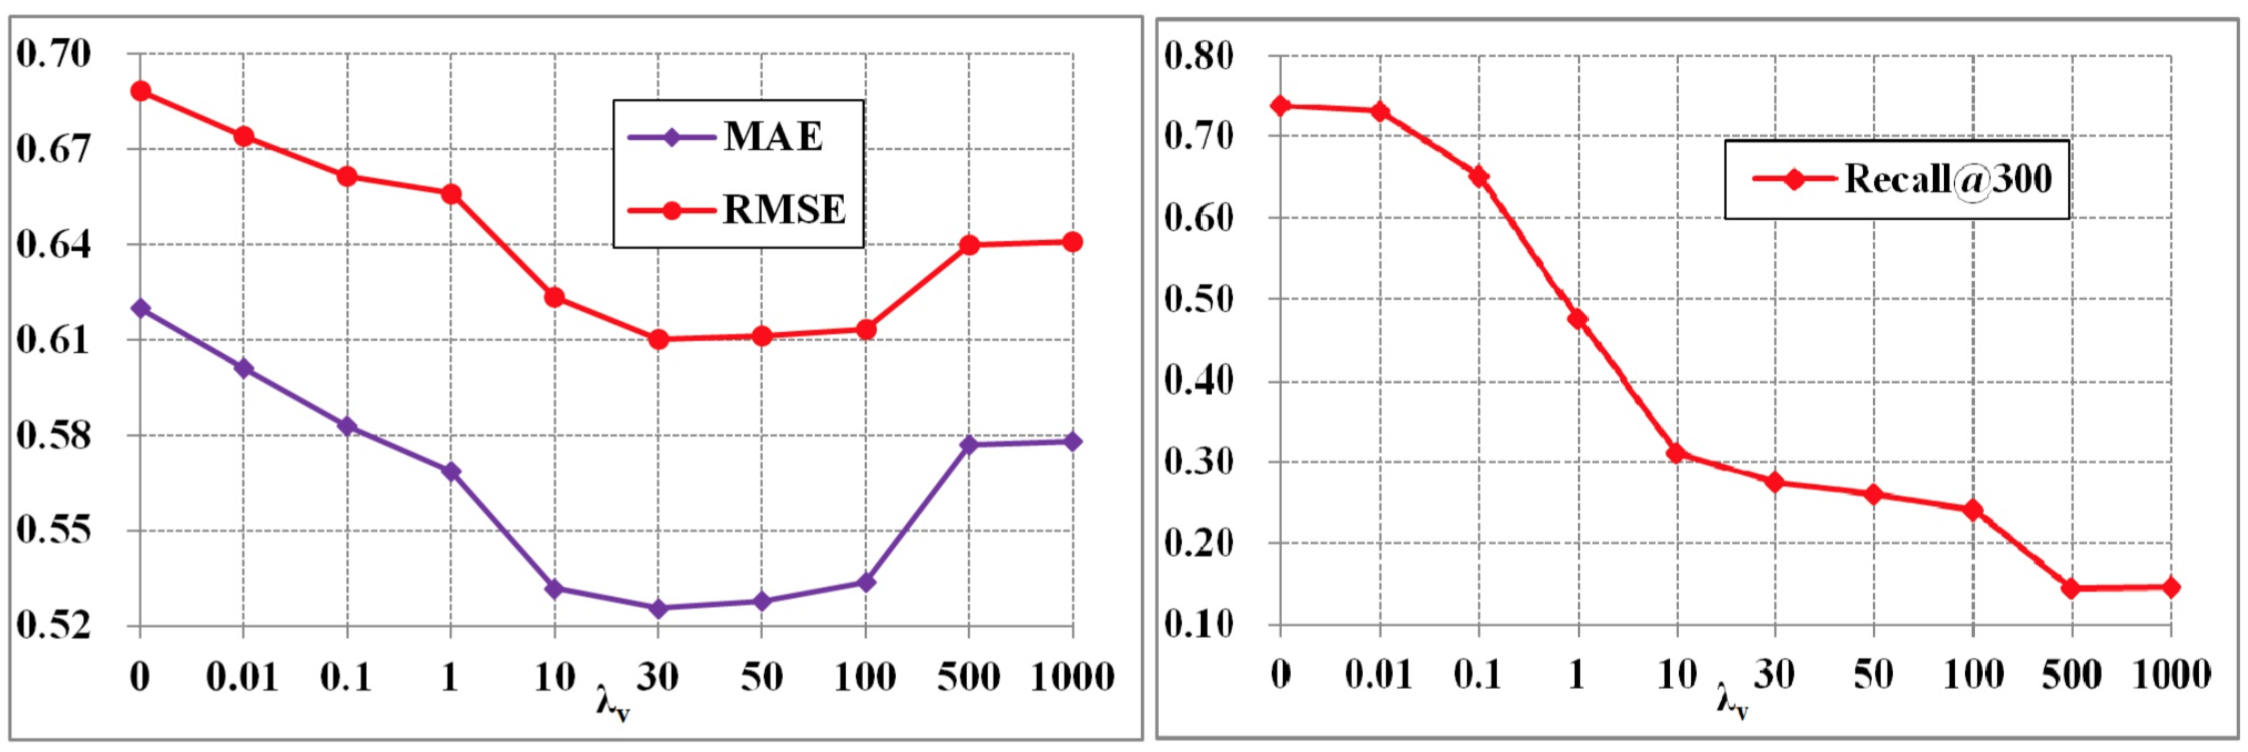
\includegraphics[width=5in]{figure2.png} 

图2:通过调节$\lambda_v$,CTR预测性能的比较。左图:MAE和RMSE,右图:recall

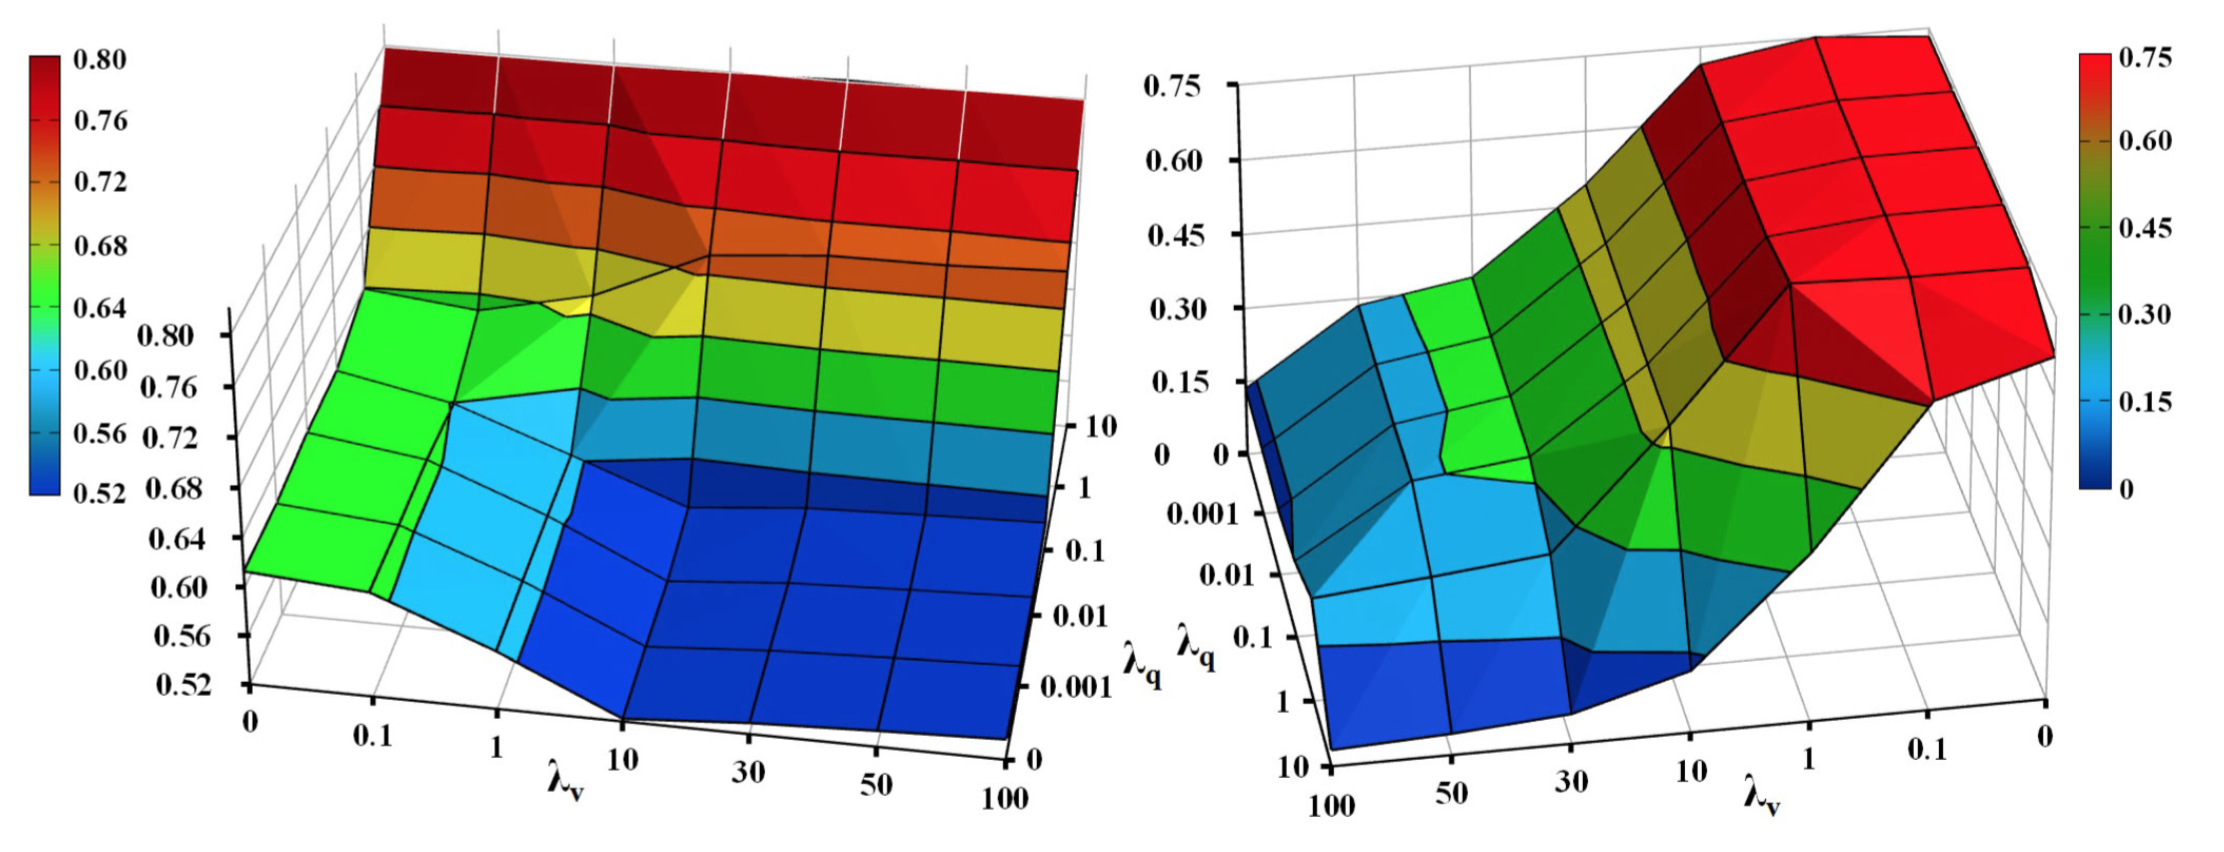
\includegraphics[width=5in]{figure3.png} 

图3:调节内容参数$\lambda_v$和社交参数$\lambda_q$获得的CTR-SMF的预测表现图,左图:MAE,右图Recall

首先,我们需要确定CTR和CTR-SMF的最佳参数。我们从图2中可以看到,当$\lambda_v = 30$和$\lambda_v = 0$,CTR达到最佳的预测的准确率和召回时。从图3我们可以看到,当$\lambda_v = 10$和$\lambda_q = 0.01$时CTR-SMF达到最好的准确性时,当$\lambda_v = 0.1$和$\lambda_q = 0$达到最佳的预测召回。

接下来,我们研究了入$\lambda_v $和$\lambda_f$对我们提出的模型C-CTR-SMF2影响。图4显示C-CTR-SMF2预测性能的三维图。内容参数平衡物品内容和评分的影响:$\lambda_v $越大,我们就更偏向于用物品内容来预测。社会参数$\lambda_f$平衡社会信任关系的影响,$\lambda_f$越大,我们就更偏向于用社会信任关系做预测。由图4可以看出,当$\lambda_v = 30,\lambda_f = 0.001$时,C-CTR-SMF2达到最佳精度预测准确性时,当$\lambda_v = 0,\lambda_f = 0.001$,达到最佳的预测召回。这表明,评分,社会关系,物品内容都有助于模型性能。

最后,我们研究了聚类数$\iota$对模型的影响。图5表明,$\iota=3$时,我们的方法达到最佳的预测精度和召回。这是因为当$\iota$第一次增加,一个类似的上下文的用户物品分组可以更好地捕捉用户的喜好,从而提供更好的性能。然而,当$\iota$超过一定的阈值($\iota=3$,在我们的数据集),推荐性能降低,因为评级矩阵的密度变得稀疏。这一结果显示基于上下文的用户物品分组效果。

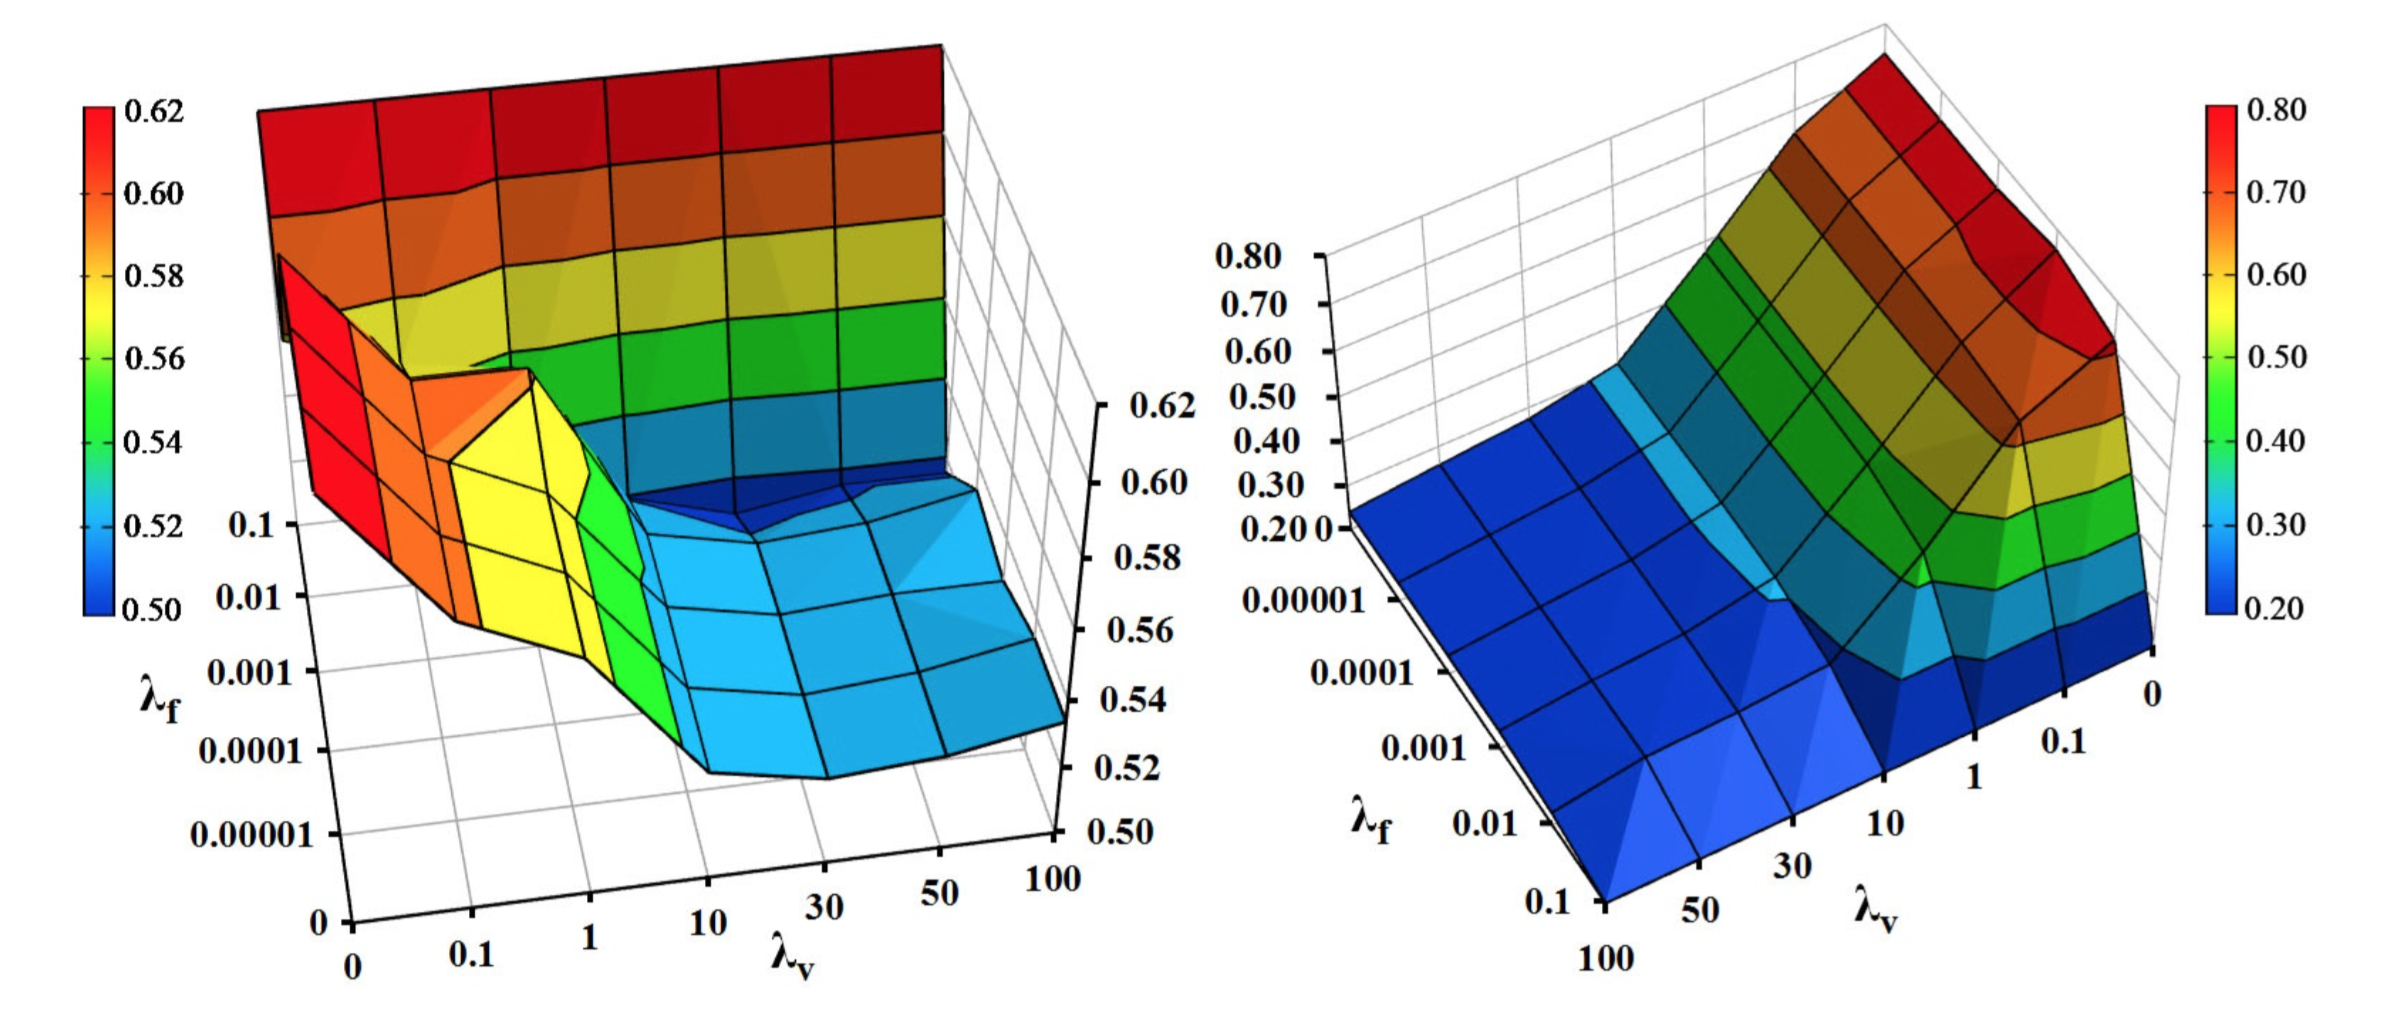
\includegraphics[width=5in]{figure4.png} 

图4:C-CTR-SMF2的预测性能图:固定$\iota$=1,改变内容参数和社会参数。左图MAE,右图recall

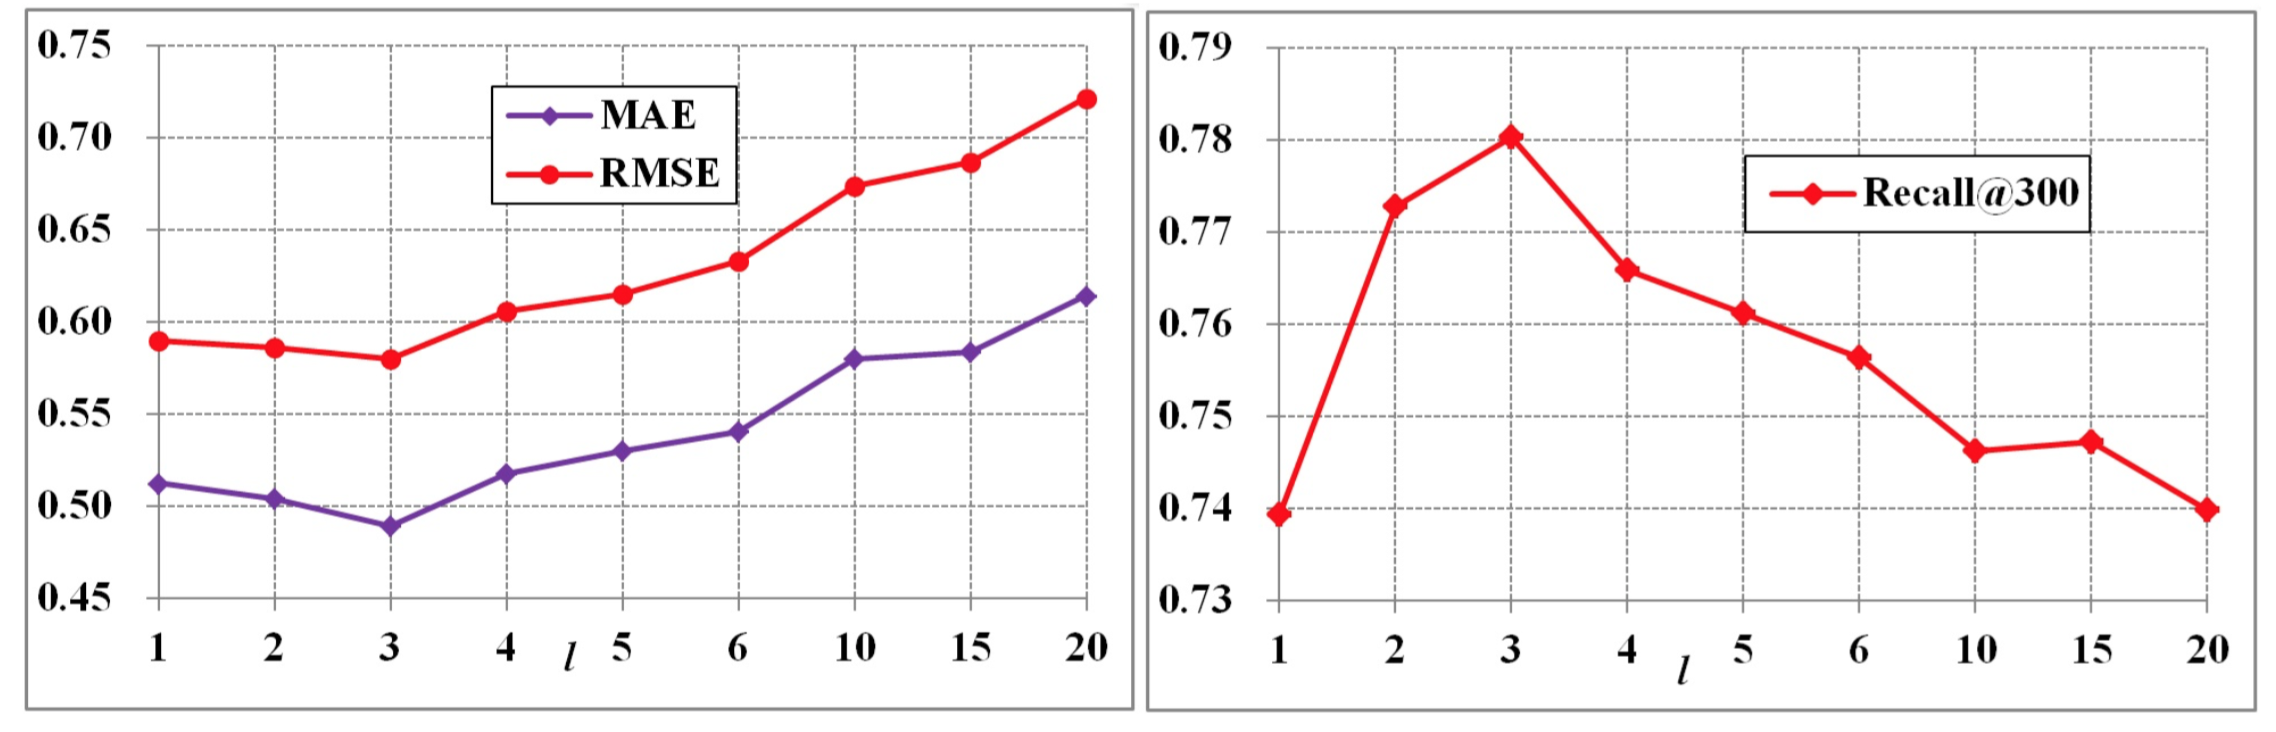
\includegraphics[width=5in]{figure5.png} 

图5:调节簇数$\iota$,获得的CTR-SMF2预测性能比较,左图MAE和RMSE,右图:recall

\subsection{性能比较与分析}
选择参数之后,我们比较了各种推荐算法在Epinions数据集模型的表现。

表1:在Epinions数据集上的性能比较

\begin{table}[!hbp]
\begin{tabular}{|c|c|c|c|c|clcl}
\hline
\hline
   & PMF & SoReg & fLDA & CTR & CTR-SMF & SoCo & C-CTR-SMF2  
\\
\hline
lMAE & 0.5629 & 0.5398 &  0.6620 & 0.5255 & 0.5212 & 0.5283 & 0.4893 
 \\
\hline
RSME & 0.6568 &  0.6211 & 0.9070 & 0.6102 & 0.5984 &  0.5988 & 0.5801
 \\
\hline
Recall & 0.3641 &  0.3641 & 0.0187 & 0.7396 & 0.7440 & 0.5666 & 0.7803
 \\
\hline
\end{tabular}
\end{table} 


分析:在所有的情况的在实验中,我们提出的方法C-CTR-SMF2表现最好。这是因为我们的模型考虑了评分、上下、社会关系和物品内容。特别是,我们采用谱聚类算法做基础用户物品分组从而可以处理分类和连续的上下文语境。同时,我们基于用户和信任他们的人的信任值,给每个用户分配不同的先验。这样,我们可以充分利用用户之间的信任,更好地反映实际情况。
\subsection{模型性能}
要看到每个类型的信息对模型性能的贡献,我们进行了以下实验:

(1) 比较C-CTR-SMF2与C-C-SMF2(在C-CTR-SMF2中设置$\lambda_v=0$)测试物品内容对预测测性能的影响。

(2)比较C-CTR-SMF2和C-R-SMF2(在C-CTR-SMF2设置$\lambda_v = \infty $)检测评分对预测性能的影响。

(3) 比较C-CTR-SMF2与C-CTR(在 C-CTR-SMF2设置$\lambda_f = 0 $)来检验社会关系对预测性能的影响。

(4) 比较C-CTR-SMF2与CTR-SMF2(设置$\iota= 1 $)测试上下文对影响的推荐预测。


图6显示C-CTR-SMF2与其他四个方法的预测性能比较,每个方法不包括一种信息。图6显示了C-C-SMF2有最坏的预测精度,说明物品内容对预测精度的影响最为显著。同样,C-R-SMF2有糟糕的recall,这表明评分对recall的影响最明显。具体而言,四种类型的信息对预测的准确性影响,降序排序:物品内容,社会关系,上细纹和评级。四种类型的信息对召回的影响,降序排序:评级,社会关系,物品内容和上下文。本实验提供了宝贵的见解,关于如何用这四种类型的信息来构建优质的RSS。

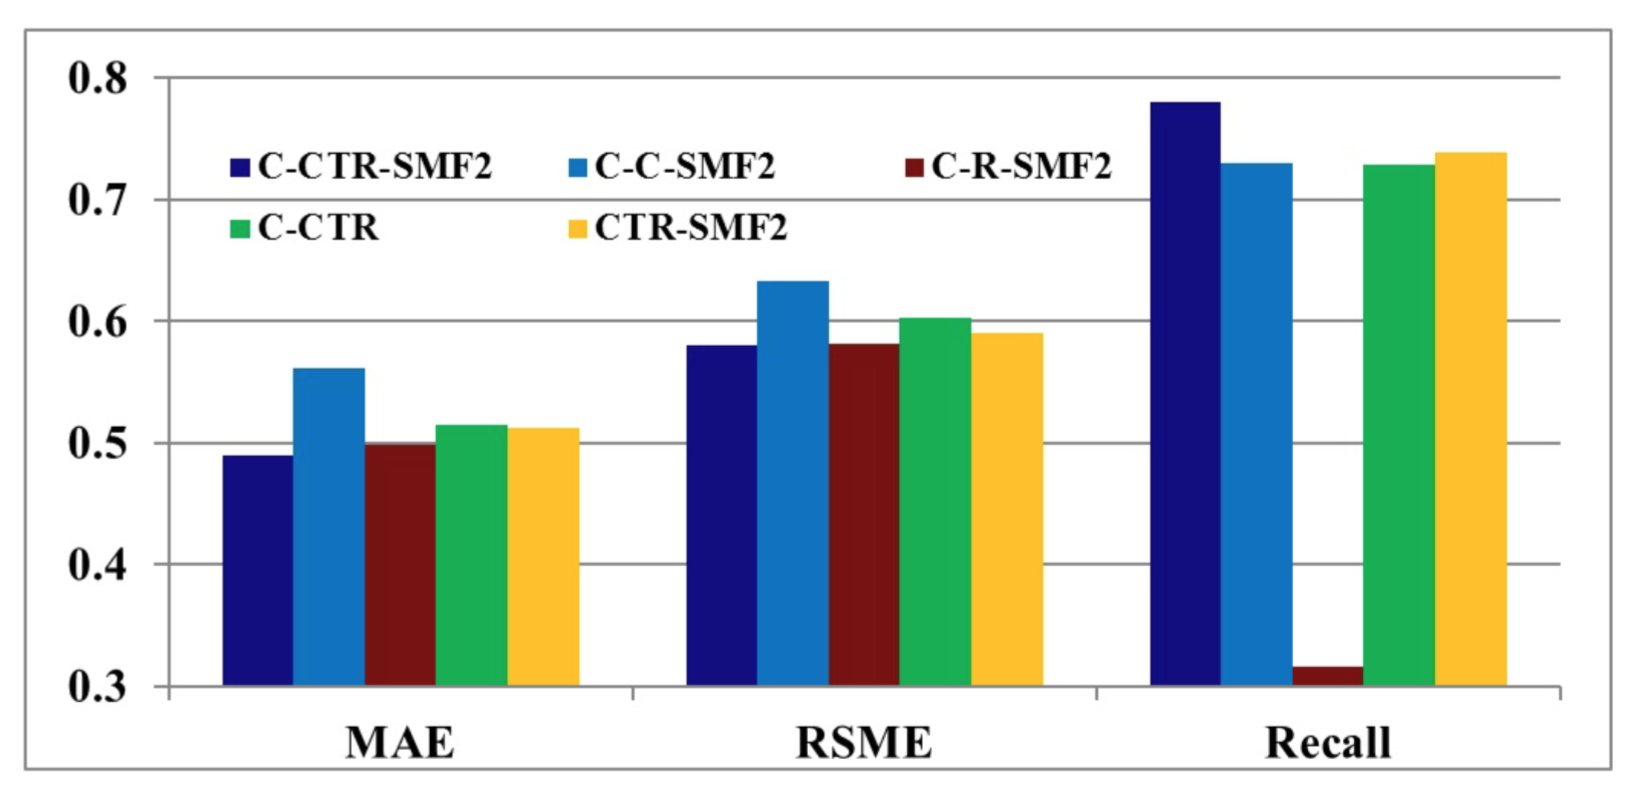
\includegraphics[width=5in]{figure6.png} 

图6:C-CTR-SMF2与其他四个方法的预测性能对比
\section{小结与讨论}
\subsection{本文总结}
本文提出了一种新的上下文感知的层次贝叶斯方法,系统结合了评级,上下文,社会关系,物品内容,以提高推荐质量。使用谱聚类为用户-物品分组,来处理分类和连续的上下文。同时,本文基于用户和信任他们的人的信任值,给每个用户分配不同的先验。在Epinions数据集上进行的实验表明,本文的方法优于六类先进的推荐方法。实验还表明,物品内容和评价分别对预测精度和召回率有着最重要的影响。

本来未来的工作将从以下两个放下考虑。一个方向考虑动态的不断变化的用户偏好。另一个方向是考虑我们的算法的并行实现,以使它们可扩展到大型数据集。
\subsection{我的体会}
1、在本文中簇数$\iota$的计算过程中,直接定义$\iota=3$时效果最佳,我觉得可以通过引入图算法中的图变化来优化这个选项

2、本文中物品主题分布$\theta$是固定的,并没有参与到训练中,我觉得可以学习$\theta$以获得更加优质的主题分布

3、可以开发增量算法,使得加入部分更新数据,不需要从头开始。

\begin{thebibliography}{MM}
\addtolength{\itemsep}{-0.5em}
\begin{small}
\bibitem{no}Chen C, Zheng X, Wang Y, et al. Context-aware collaborative topic regression with social matrix factorization for recommender systems[C]//Twenty-Eighth AAAI Conference on Artificial Intelligence. 2014.
\end{small}
\end{thebibliography}
\newpage
%\end{xeCJK}
\end{document}

